\section{Operations and Logistics}
\label{OperationsLogistics}

In order for the laser swarm to be successful it has to operate efficiently and effectively, so that the obtained surface model and other data can be sold on the market. This chapter will consider some of these operations and their required logistics. Note that only operations after successful orbit injection and deployment, and before the \ac{EOL} are considered. A graphical representation of the hierarchy of the options considered here can be found in figure \ref{fig:OpsHier} on page \pageref{fig:OpsHier}.

\begin{figure}
\centering
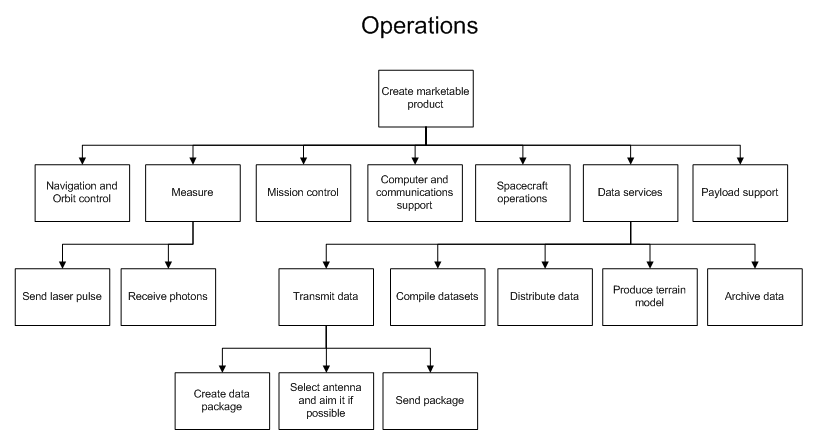
\includegraphics[width=1.0\textwidth, angle=0]{chapters/img/OpsHierarchy.png}
\caption{Hierarchy of the operations for the laser swarm mission.}
\label{fig:OpsHier}
\end{figure}

Navigation and orbital control is an important operation for the laser swarm mission. For example, without an accurate knowledge of the position of the satellites the gathered data is useless and orbital control cannot be performed. All satellites use a \acs{GPS} receiver to determine their position up to about one meter. Orbital control is performed automatically based on the received \acs{GPS} data. It is clear by now that this system is to work automatically, however it is important there are people on the ground who check for any anomalies and give corrections whenever necessary.

Mission control entails the real time control of the satellites. However because the mission is automated the amount of people for mission control can be limited. The only active inputs by humans are commands sent to the satellite to correct for any errors that may occur.

The measurements will be performed completely autonomously, with human inputs only being used to correct an error in the automation or to change the mission routine. The measuring operation includes the both the emitter and the receivers, for a greater detail of the functions that have to be performed the function flow diagram in section \ref{section_FFD} may be consulted.

Payload support is comprised of one or more people who monitor the condition and performance of the laser payload, and a separate group of people who monitor the receiving payload on both the emitter and receiver satellites. In case of an anomaly they determine the severity and adjust the payload operations or satellite functioning to correct the problem.

Spacecraft operations is similar to payload support, except that the person or people who work on this operation monitor the other subsystems of the satellite by analyzing the housekeeping data from the payloads, navigational systems, the power subsystems or the antennae to name some examples.

Computer and communications support has a staff of several people who monitor the onboard computer of the satellites and the system automation, and one or two persons who monitor the communications between satellites and from the emitter satellite to the ground. Their main job is to ensure the system remains operational if an anomaly occurs.

Data services entails everything that happens with all data both on ground and aboard the satellites. The data can be anything from measurement data to navigational data and housekeeping data. This operation supports all others. While largely automated some human interaction is needed to ensure the data in decoded, debugged, archived and generally handled properly. Minimal human interaction should be required to reduce the mission costs.

Data transmission involves the sending of data between satellites and from the satellites to a ground station. The satellites will use their position and attitude data to determine which antenna to use for intersatellite communication, and the emitter will perform a similar operation using its own position and attitude data direct communications to the ground station. This process is fully automated, and a failure in the X-band phased array means that a ground station will have to aim towards a receiver satellite in order to attempt to fix the problem. So normally this operation requires no personnel, but in case of failure several persons are required to attempt to save the mission.